\section{Method}

\subsection{Experiment Design}

We hypothesized that with a procedural learning technique users will find it easier to learn an unfamiliar optimized keyboard layout and be more willing to use the new keyboard regularly.  Our idea is to begin the study with a Qwerty keyboard and over time switch a few keys until the user gets used to it.  That process will continue until all of the keys are in their fully optimized position.

In this field study we have a control group and an experimental group.  The control group will be told to use the completed optimized keyboard while the experimental group will be given the Qwerty keyboard that changes over time.  

The main instrumentation we are using in this study is the keyboard application that we are downloading onto our subjects' phones. Once we collect our sample, we will set up times to meet with them to explain the study and application.  Before they get started, we want to take preliminary measurements on their use with the Qwerty keyboard before we switch it around. This will give us an idea of how they improve or decline throughout the course of the study.  

Our participants will be asked to use our keyboard as their native keyboard during the study, and they will periodically receive alerts to test their progress with the keyboard.   In order to test their progress they will need to go into out application and copy a line of text that is displayed.  The application will store the measurements taken.


We will be updating the application's keys for each participant after they complete \gdc{some number} check points.   \gdc{(NEEDS JUSTIFICATION)} We noticed, on the keyboard, that certain groups of keys are all switched with each other.  The groupings vary from twelve keys to two keys.  The two-key sets make it easy to figure out which keys to switch.  They twelve-key group, however, will have to be split into about four to six smaller groupings to allow for ease of learning for the participants.  

Below is our initial idea of how we want to switch the keys around on the Quasi-Qwerty keyboard.  The first three key switches are groupings of two. The next three switches are a key grouping of four that is split into multiple different switching stages. Similarly, the last group of key alterations is from a group of 7 keys.  There are also the key replacements for the Sath-Trap keyboard.  The first two replacements listed were groupings of two.  The third was a key grouping of three and the replacements below the line was a grouping of twelve that was split up into five different replacements.  



\begin{figure*}[ht]
	\centering
	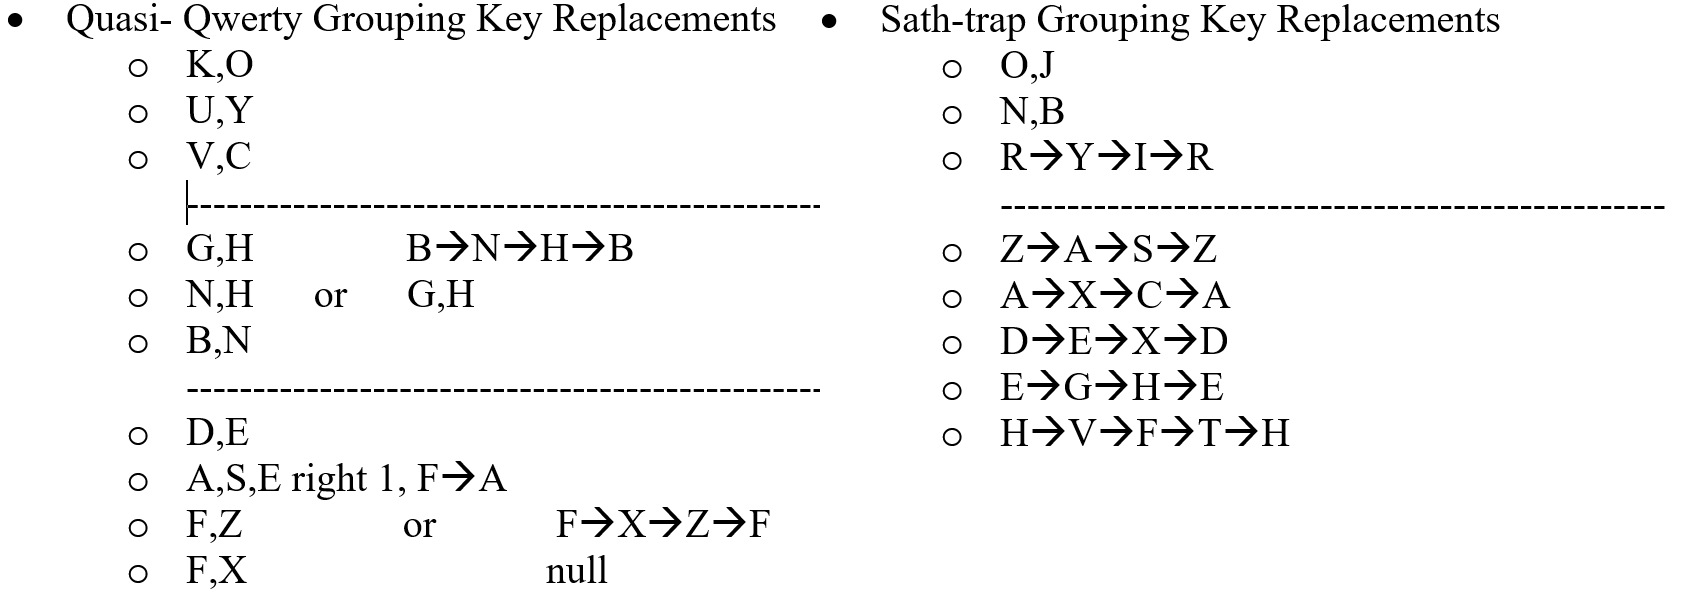
\includegraphics [width=0.8\linewidth]{figures/group1}
	
\end{figure*}

An alternative method we are considering for key replacement is initially moving the vowels to heir place on the new keyboard. Next, we will swap keys to their respective places beginning from Q, in the top left corner, and working our way to M, in the bottom left corner.  Below are the replacements for this method.  


\begin{figure*}[ht]
	\centering
	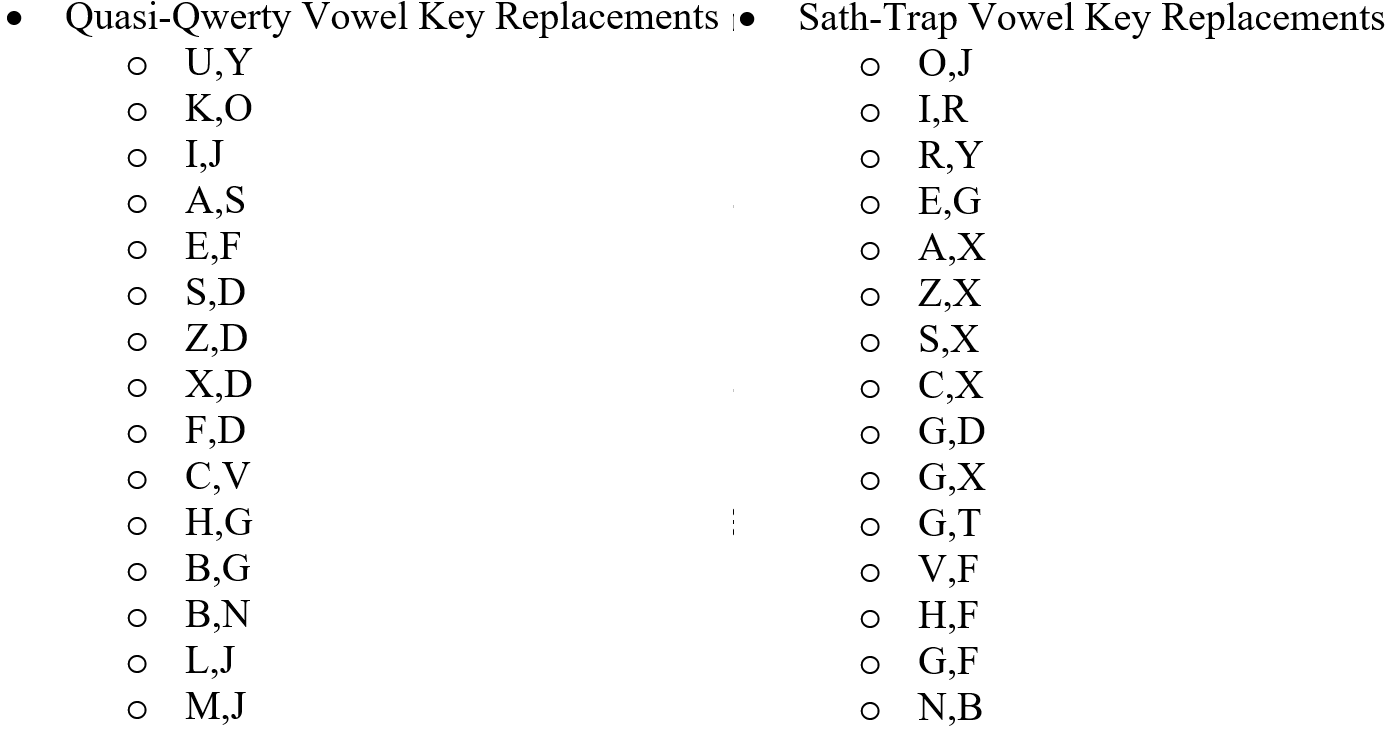
\includegraphics [width=0.7\linewidth]{figures/group2}
	
\end{figure*}


\subsection{Measurement}

The main instrumentation we are using in this study is the keyboard application that we are downloading onto our subjects' phones. In this experiment we are still trying to narrow down what metrics we want to use.  Some of the options discussed are: 

\begin{itemize}
\item Speed in words per minute (WPM)[2].  This measurement regards every five characters typed as one word, including spaces. This measurement includes the length of the transcribed string excluding the first letter, divided by the time in seconds it took to type that string.  Then, multiply by 60 to convert the seconds to minutes and divide by five to convert number of characters to number of ‘words'.  

\item Accuracy (Corrected, uncorrected, or total error rates) [2].  This measurement includes correct characters (C), incorrect and not fixed characters (INF), incorrect and fixed characters (IF) and finally all backspaces used to fix errors (F). Using these variables, you can calculate three different error rates; corrected, uncorrected, and total.  Corrected error rate is IF/(C+INF+IF), uncorrected error rate is INF/(C+INF+IF), and total error rate is the sum of the two.  

\item Error rates can also be measured by Cumulative and Chunk error rates [2].  This method would disallow error correction all together and treated any character out of place as an error.  The use of this measurement would require the users to be copying a display text that is presented to them.  

\item Efficiency measures can include utilized bandwidth, and wasted bandwidth [2]. Utilized bandwidth is the measure of how many correct characters there are in comparison to the whole transcribed string: C/(C+INF+IF+F).  Wasted bandwidth is the opposite: (INF+IF+F) /(C+INF+IF+F).  

\item Efficiency can also be measured in cost per correction (CPC).  This measurement accounts for errors that were made but not noticed immediately.  CPC is defined by (IF+F)/(Corrections).  A correction is the number of consecutive chunks of backspaces and letters.  There can be one correction in a string, and there can be multiple corrections in a string.  

\item Initial Entry Time [6]- The time between when a word is presented on the screen to when the last letter in that word is typed.  This measures the user's ability to find the keys quickly.
\end{itemize} 
